\section{Applied Perception II }
\subsection{Color Vision}
La \textit{Color Vision} può essere considerata come superflua nella vita moderna
Ma il colore comunque è estreamamente utile nella data visualization:
\begin{itemize}
    \item Mostrare i patterns
    \item Labeling
    \item Mettere in evidenza
\end{itemize}
\begin{figure}[H]
    \centering
    \begin{minipage}{0.45\textwidth}
        \centering
        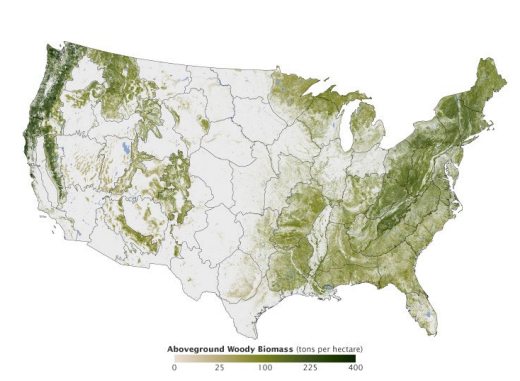
\includegraphics[width=\linewidth]{images/ColorVision.png} 
        \caption{Effetti della color vision}
        \label{fig:immagine1}
    \end{minipage}\hfill
    \begin{minipage}{0.45\textwidth}
        \centering
        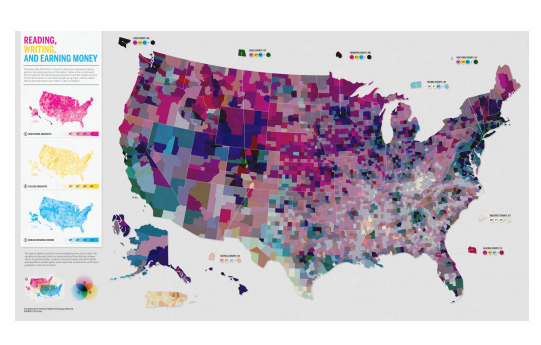
\includegraphics[width=\linewidth]{images/ColorVision2.png} 
        \caption{Effetti della color vision}
        \label{fig:immagine2}
    \end{minipage}
\end{figure}
Pensare al colore come un attributo di un oggetto invece che ad una caratteristica primaria(C.Ware).
\subsection{Trichromacy and Opponent process theories}
Abbbiamo, sulla retina, tre distinti recettori per i colori:
\begin{itemize}
    \item the \textbf{cones}: che sono attivi ai livelli normali di luce
    \item the \textbf{rods}: l'influenza dei rods sulla percezione può essere ignorata.
\end{itemize}
\subsubsection{Trichromacy theory}
I \textit{cones} sono sensibili alle diverse onde di luce.
Quindi, assorbono luce attorno lo spettro del colore blue, verde e rosso.
La teoria dice che percepiamo il colore tramite un sistema a tre canali.
Tutti gli spazi dei colori, anche se progettati per scopi diversi, sono tridimensionali.
\begin{figure}[H]
    \centering
    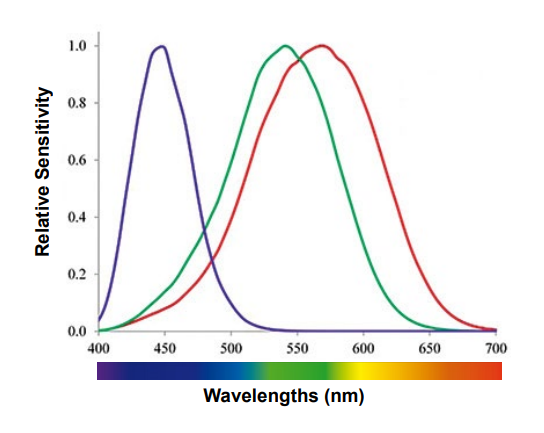
\includegraphics[width=0.5\textwidth]{images/Thrichromacy.png} 
    \caption{Trichromacy theory}
    \label{fig:immagine}
\end{figure}
\subsubsection{colour measurement and specifcation}
Dato che solo tre diversi recettori sono coinvolti nella colori vision, è possibile fare il match dei colori
usando un mix di tre colori, chiamati primari.
Dato uno standard di colori primari, si può usare una transformazione per creare lo stesso colore in output in device diversi 
\begin{figure}[H]
    \centering
    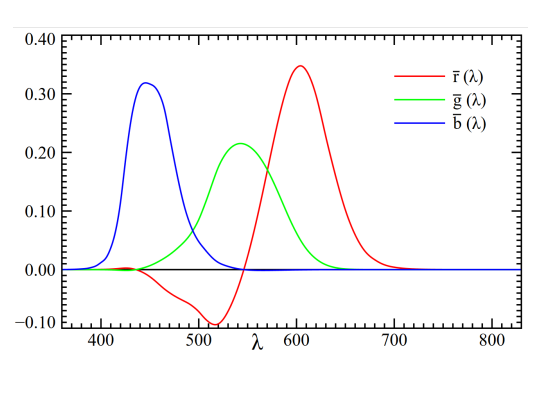
\includegraphics[width=0.5\textwidth]{images/RGB.png} 
    \caption{RGB color Matching Function}
    \label{fig:immagine}
\end{figure}
\subsubsection{CIE XYZ Color Space}

Lo spazio colore CIE XYZ è uno spazio colore standardizzato sviluppato dalla Commission Internationale de l'Eclairage (CIE). È un modello matematico che rappresenta tutti i colori visibili agli esseri umani attraverso tre valori numerici: X, Y e Z.
Questi valori sono definiti in base alle risposte dei tre tipi di coni presenti nell'occhio umano (sensibili alle lunghezze d'onda dei colori rosso, verde e blu).
Il valore Y rappresenta la luminosità, mentre X e Z descrivono la posizione orizzontale e verticale del colore nello spazio XYZ.
 
Il diagramma di cromaticità è uno strumento visivo utilizzato per rappresentare i colori visibili senza tener conto della luminosità. Questo diagramma rappresenta le proprietà del colore in termini di tonalità e saturazione, ignorando la luminanza.
\subsubsection{Opponent process theory}

Alla fine del XIX secolo, il psicologo tedesco Hering propose la teoria (successivamente supportata da prove sperimentali) secondo cui i coni della retina combinano il loro stimolo formando tre coppie di colori che competono tra loro per formare quello finale. Queste coppie, chiamate coppie antagoniste, sono: nero-bianco, giallo-verde e giallo-blu
\textbf{Evidenze a supporto della teoria:}
\begin{itemize}
  \item Nomenclatura
  \item Tonalità uniche
  \item Neurofisiologia
\end{itemize}

\textbf{Proprietà dei canali di colore antagonisti:}
\begin{itemize}
  \item Risoluzione spaziale
  \item Percezione della forma
  \item Contrasto cromatico
\end{itemize}

La teoria della tricromia e la teoria dei colori antagonisti operano a livelli differenti.

La teoria della tricromia spiega ciò che accade a livello dei fotorecettori.
La teoria dei colori antagonisti spiega ciò che accade a livello neurale.
\subsection{Color Space}
\subsubsection{RGB Color Space}

Lo spazio dei colori \textbf{RGB} (Red, Green, Blue) è un modello di colore utilizzato comunemente nel contesto digitale e dell'informatica per rappresentare i colori. Questo spazio dei colori si basa sulla combinazione di tre colori primari: rosso (Red), verde (Green) e blu (Blue).
Nel modello RGB, ogni colore può essere rappresentato come una combinazione di intensità di questi tre colori primari. Ogni colore è rappresentato da un punto in uno spazio tridimensionale dove i tre assi corrispondono a rosso, verde e blu.
La combinazione di diverse intensità di rosso, verde e blu consente di ottenere una vasta gamma di colori. Ad esempio, il nero si ottiene quando tutte e tre le componenti (R, G, B) sono al minimo, mentre il bianco si ottiene quando tutte e tre
 sono al massimo. I colori primari (rosso, verde e blu) sono usati come base per creare tutti gli altri colori nel modello RGB.
\begin{figure}[H]
    \centering
    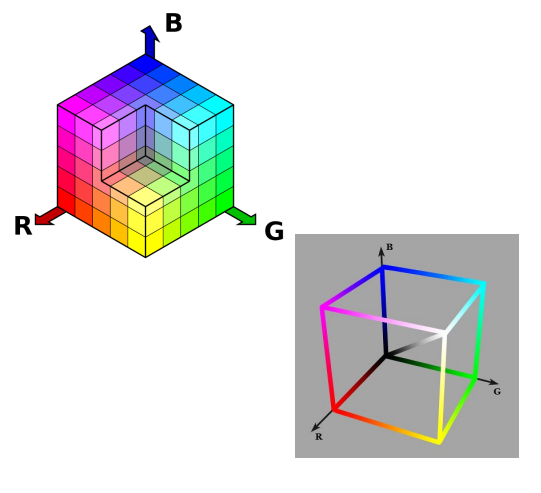
\includegraphics[width=0.5\textwidth]{images/RGBCOlor.png} 
    \caption{RGB color}
    \label{fig:immagine}
\end{figure}
\subsubsection{HSV/HSL color space}

\textbf{HSV} (Hue, Saturation, Value) e \textbf{HSL} (Hue, Saturation, Lightness) sono due modelli di spazio dei colori correlati che rappresentano i colori in termini di tre componenti principali: tonalità (Hue), saturazione (Saturation) e valore o luminosità (Value per HSV, Lightness per HSL).
La specifica del colore risulta essere più intuitiva con HSV/HSL rispetto a RGB. Tuttavia, questi spazi di colore non sono uniformi dal punto di vista percettivo, il che implica che le distanze calcolate all'interno dello spazio colore 
non corrispondono alle distanze percettive.
\subsubsection{CIE Lab/Lch color space}
Lo spazio colore CIE Lab/Lch è un sistema di colore sviluppato dalla Commissione Internazionale dell'Illuminazione (CIE). Questo spazio colore è progettato per rappresentare i colori in modo più uniforme e vicino alla percezione umana rispetto ad altri spazi 
colore come RGB, HSV o HSL.
\subsubsection{Color differences}
Avere uno space color in cui le distanze percettive uguali corrispondono a distanze uguali è utile per specificare tolleranze del colore, codici colore, pseudocolore (utilizzando sequenze di colori per rappresentare valori dei dati, possibilmente con passaggi percettivamente uguali).
Anche se gli space color uniformi forniscono solo un'approssimazione iniziale approssimativa di come saranno percepite le differenze di colore, un fattore influente importante è la dimensione (siamo molto più sensibili alle differenze tra grandi campi).
Suggerimento: utilizzare colori saturi quando si codifica piccoli simboli o linee sottili e colori meno saturi per aree grandi.
\begin{figure}[H]
    \centering
    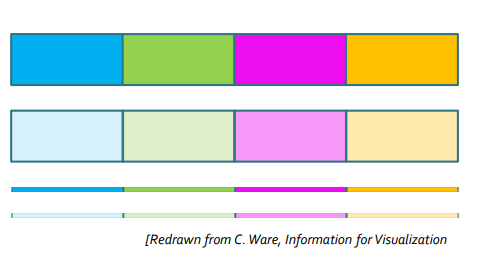
\includegraphics[width=0.5\textwidth]{images/ColorDifferences.png} 
    \caption{Color differences}
    \label{fig:immagine}
\end{figure}
\subsection{Color and visualization}
\subsubsection{Luminance and visualization}
I canali cromatici rosso-verde e giallo-blu sono in grado ciascuno di trasportare 
solo circa un terzo della quantità di dettagli trasportati dal canale in bianco e nero (Mullen, 1985). 
Le differenze puramente cromatiche non sono sufficienti per visualizzare dettagli fini. Assicurare un adeguato contrasto di luminanza con lo sfondo (anche se vengono utilizzati colori con differente cromaticità).
Un confine di contrasto può migliorare la leggibilità dei simboli colorati.
\subsubsection{Saturation and visualization}
Utilizzare colori saturi per codificare piccoli simboli/dettagli fini e colori meno saturi per codificare aree grandi.
\subsubsection{Color for Labeling}
Post e Greene (1986) hanno condotto un esperimento sulla denominazione dei colori (sono stati mostrati 210 colori diversi su uno sfondo nero in una stanza oscurata). Solo otto colori più il bianco vengono denominati in modo coerente. Anche se non è generalmente applicabile,
ciò suggerisce che solo pochi colori possono essere utilizzati come etichette di categoria.
\subsubsection{Color and semantics}
Fai attenzione alle convenzioni dei colori e alle associazioni semantiche (rosso per caldo/cattivo/pericolo, blu per freddo, verde per vita/vai, ecc.), 
poiché le convenzioni non sono universali. L'associazione semantica con il grigio è quella di appartenenza a una categoria non specificata (utile per evidenziare)
Evita colori problematici per le persone daltoniche.
Utilizza una scala di colori basata sullo spettro solo quando il suo utilizzo è profondamente radicato nella cultura degli utenti.
Per rivelare dettagli fini, utilizza sequenze di pseudocolori che variano nella luminosità, non solo nella cromaticità.